\documentclass[12pt,a4paper]{leaflet}
\usepackage[T1]{fontenc}
\usepackage[utf8]{inputenc}
\usepackage[portuges]{babel}
\usepackage{color,flowfram,graphicx}
\usepackage{wrapfig,rotating}
\usepackage{multirow,multicol,array,mathpazo}
\usepackage{titlesec}
\usepackage{framed,libertine}
\usepackage[usenames,dvipsnames,svgnames]{xcolor}
\usepackage{amssymb}
\usepackage{subcaption}
\usepackage{enumitem}
\usepackage{setspace,fontawesome} %fb and youtube icon
\usepackage[colorlinks=true, urlcolor=black]{hyperref}
\urlstyle{same}

\definecolor{escurode}{HTML}{001132} 
\definecolor{clarode}{HTML}{083765}
\definecolor{laranjade}{HTML}{FF0007}
\definecolor{amarelode}{HTML}{FFFC00}
\titleformat*{\section}{\huge\bf\color{escurode}}

\renewcommand{\labelitemi}{$\textcolor{laranjade}{\blacktriangleright}$}
\renewcommand{\labelitemii}{$\textcolor{clarode}{\blacktriangleright}$}
\renewcommand{\labelitemiii}{$\textcolor{escurode}{\blacktriangleright}$}
\renewcommand{\theenumi}{\color{laranjade}{\arabic{enumi}}}
\renewcommand{\theenumii}{\color{clarode}{\alph{enumii}}}
\renewcommand{\theenumiii}{\color{escurode}{\roman{enumiii}}}

\newcommand{\destacado}[2]{\textcolor{#1}{\textbf{#2}}}

\newcommand*\openquote{\makebox(25,-22){\scalebox{5}{``}}}
\newcommand*\closequote{\makebox(25,-22){\scalebox{5}{''}}}

\colorlet{shadecolor}{escurode}

\makeatletter
\newif\if@right
\def\shadequote{\@righttrue\shadequote@i}
\def\shadequote@i{\begin{snugshade}\begin{quote}\openquote}
\def\endshadequote{%
  \if@right\hfill\fi\closequote\end{quote}\end{snugshade}}
\@namedef{shadequote*}{\@rightfalse\shadequote@i}
\@namedef{endshadequote*}{\endshadequote}
\makeatother

%FONT Change
%\renewcommand{\familydefault}{cmss} 

% To draw a horizontal Line
\newcommand{\sectionline}{
 \nointerlineskip \vspace{\baselineskip}
 \hspace{\fill}\rule{0.8\linewidth}{.7pt}\hspace{\fill}
 \par\nointerlineskip \vspace{\baselineskip}
}


% Make a border along the top of each page
\setmargins{15mm}{15mm}{7mm}{7mm}
\vtwotonetop{1cm}{0.6\paperwidth}{[cmyk]{0.96,0.97,0.56,0.46}}{topleft}{0.4\paperwidth}{[cmyk]{0.96,0.97,0.56,0.46}}{topright}
\vtwotonebottom{1cm}{0.6\paperwidth}{[cmyk]{0.96,0.97,0.56,0.46}}{bottomleft}{0.4\paperwidth}{[cmyk]{0.96,0.97,0.56,0.46}}{bottomright}

% \pagestyle{empty}



\begin{document}

\begin{titlepage}
\title{
\Huge\color{escurode}
	\textbf{Departmento de Estatística da UFPB}
}
\date{}
\end{titlepage}


\maketitle

Nosso Bacharelado em Estatística é \destacado{laranjade}{jovem}, tendo sido fundado em 2000. Nossa primeira turma se graduou no primeiro semestre de 2004. No momento contamos com:


\begin{itemize}
    \item 27 professores
    \item 124 estudantes ativos
    \item Um proggrama de Pós-Graduação interdisciplinar com cursos de Mestrado e Doutorado
    \item 8 \destacado{laranjade}{laboratórios dedicados} %%%%%%%%%%%%%%%%% IMPORTANTE: O comando destacado recebe primeiro uma cor (escurode, clarode, laranjade, amarelode) e depois o texto destacado %%%%%%%%%%%%%%%%%
    
\end{itemize}

\begin{center}
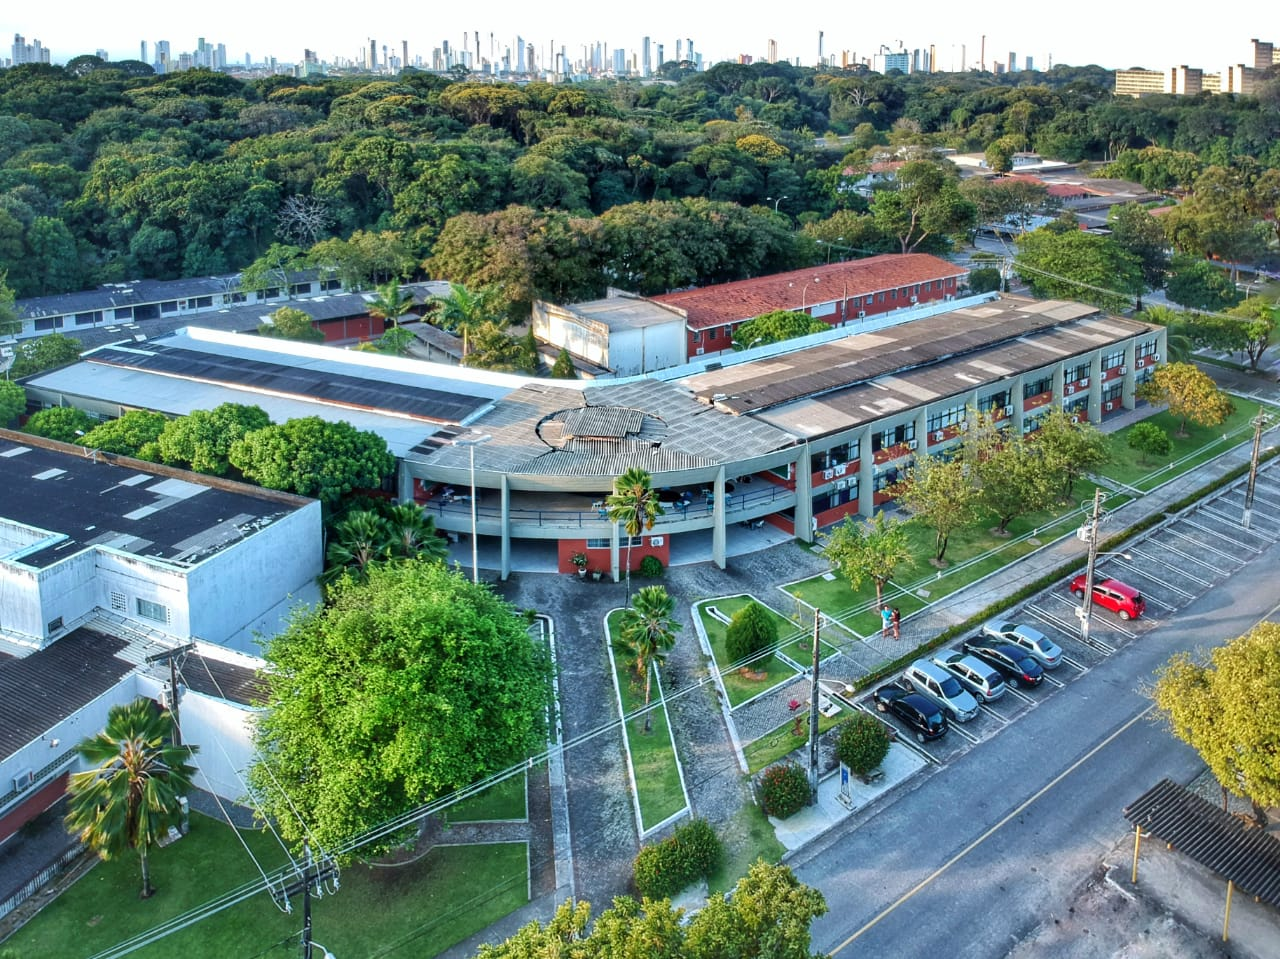
\includegraphics[width=0.9\textwidth]{figuras/bumerangue.jpg}
\end{center}

\newpage

\section{Outra Seção}

Texto de uma outra seção

\newpage

\section{}

Esta Seção não tem título


\newpage

\section{Última Seção}

    \begin{enumerate}
        \item Um item
        \begin{enumerate}
            \item Um sub-item
            \begin{enumerate}
                \item Um sub-sub-item
                \item Outro sub-sub-item
            \end{enumerate}
            \item Outro sub-item
        \end{enumerate}
        \item Outro item
    \end{enumerate}

\newpage

\section{Uma Seção}

Um texto de seção.
    
    \begin{itemize}
        \item Um item
        \item Outro item
        \begin{itemize}
            \item Um sub-item
            \begin{itemize}
                \item Um sub-sub-item
            \end{itemize}
        \end{itemize}
    \end{itemize}

\newpage

\section{Quer saber mais?}
Segue a gente nas redes sociais:

\begin{table}[h]
\begin{tabular}{ll}
\raisebox{-\totalheight}{
\includegraphics[width=0.06\linewidth]{figuras/Instagram_icon.png}}         &   \raisebox{-\totalheight}{\destacado{clarode}{@estatisticaufpb}}\\
\raisebox{-\totalheight}{
\includegraphics[width=0.06\linewidth]{figuras/facebook-logo.png}}                        &  \raisebox{-\totalheight}{\destacado{clarode}{Grupo Estatística - UFPB}} \\

\end{tabular}
\end{table}

Ou acesse \destacado{clarode}{\underline{www.de.ufpb.br}}

\vfill
\begin{center}

\includegraphics[width=0.9\textwidth,trim={3.2cm 0 2.7cm 0},clip]{figuras/logo-texto.png}

\footnotesize{
	\textcopyright\ 2019 Departamento de Estatística | 
    	Universidade Federal da Paraíba
        }
\end{center}

\end{document}